% !TEX TS-program = pdflatex
% !TEX encoding = UTF-8 Unicode

% This is a simple template for a LaTeX document using the "article" class.
% See "book", "report", "letter" for other types of document.

\documentclass[11pt]{article} % use larger type; default would be 10pt

\usepackage[utf8]{inputenc} % set input encoding (not needed with XeLaTeX)

%%% PAGE DIMENSIONS
\usepackage{geometry} % to change the page dimensions
\geometry{a4paper} % or letterpaper (US) or a5paper or....

\usepackage{graphicx} % support the \includegraphics command and options

\usepackage{amssymb}
\usepackage{amsmath}
%%% PACKAGES
\usepackage{booktabs} % for much better looking tables
\usepackage{array} % for better arrays (eg matrices) in maths
\usepackage{paralist} % very flexible & customisable lists (eg. enumerate/itemize, etc.)
\usepackage{verbatim} % adds environment for commenting out blocks of text & for better verbatim
\usepackage{subfig} % make it possible to include more than one captioned figure/table in a single float
% These packages are all incorporated in the memoir class to one degree or another...

%%% HEADERS & FOOTERS
\usepackage{fancyhdr} % This should be set AFTER setting up the page geometry
\pagestyle{fancy} % options: empty , plain , fancy
\renewcommand{\headrulewidth}{0pt} % customise the layout...
\lhead{}\chead{}\rhead{}
\lfoot{}\cfoot{\thepage}\rfoot{}

%%% SECTION TITLE APPEARANCE
\usepackage{sectsty}
\allsectionsfont{\sffamily\mdseries\upshape} % (See the fntguide.pdf for font help)
% (This matches ConTeXt defaults)

%%% ToC (table of contents) APPEARANCE
\usepackage[nottoc,notlof,notlot]{tocbibind} % Put the bibliography in the ToC
\usepackage[titles,subfigure]{tocloft} % Alter the style of the Table of Contents
\renewcommand{\cftsecfont}{\rmfamily\mdseries\upshape}
\renewcommand{\cftsecpagefont}{\rmfamily\mdseries\upshape} % No bold!

\usepackage{amsmath}
\usepackage{graphicx}
\graphicspath{ {./pings/} }
\DeclareMathOperator*{\argmax}{arg\,max}
\DeclareMathOperator*{\argmin}{arg\,min}

\newcount\colveccount
\newcommand*\colvec[1]{
        \global\colveccount#1
        \begin{pmatrix}
        \colvecnext
}
\def\colvecnext#1{
        #1
        \global\advance\colveccount-1
        \ifnum\colveccount>0
                \\
                \expandafter\colvecnext
        \else
                \end{pmatrix}
        \fi
}

%%% END Article customizations

%%% The "real" document content comes below...

\title{Micro HW1}
\author{Michael B. Nattinger\footnote{I worked on this assignment with my study group: Alex von Hafften, Andrew Smith, Ryan Mather, and Tyler Welch. I have also discussed problem(s) with Emily Case, Sarah Bass, and Danny Edgel.}}

%\date{} % Activate to display a given date or no date (if empty),
         % otherwise the current date is printed 

\begin{document}
\maketitle

\section{Question 1}
Let $t_i \in S_i$ be strictly dominated by some (potentially mixed) strategy $\sigma'_i \in \Delta S_i$. Then let $\sigma_i$ be some mixed strategy with $t_i$ in its support. Then, for some $p \in (0,1],$ $\sigma_i = p t_i + (1-p) \sigma^{*}_i$ for some $\sigma^{*}_i \in \Delta S_i.$ Then, $u(\sigma_i) = u( p t_i + (1-p) \sigma^{*}_i) < u( p \sigma'_i + (1-p) \sigma^{*}_i)$ so $\sigma_i$ is strictly dominated.
\section{Question 2}
\subsection{Part A}
$N = \{ 1,2\}$. Each traveler chooses from $s_i = \{ 2,3,\dots ,500 \}$. The payoff function is $u_i(s_i,s_{-i}) = \begin{cases} s_i, s_i = s_{-i} \\ s_i+2, s_i<s_{-i}  \\ s_{-i}-2, s_{-i}<s_i \end{cases}$.
\subsection{Part B}
If player 1 believes that the highest action in $S_2$ that receives positive probability is $\bar{s}_2>0$, player 1's best response is less than  $\bar{s}_2>0$. We can show this in the following way:

Say player 1 believes that the highest action in $S_2$ that receives positive probability is $\bar{s}_2>0$. Say player 1 chooses $\bar{s}$ themselves. Then, their expected payoff is $EP(\bar{p}_2) = p_{\bar{s}_2} \bar{s}_2 + \sum_{i\neq \bar{s}_2} p_i i-2 <p_{\bar{s}_2} (\bar{s}_2+1) + \sum_{i=1}^{\bar{s}_2 -1} p_i i-2 \leq p_{\bar{s}_2} (\bar{s}_2 +1) +  p_{\bar{s}_2 -1} (\bar{s}_2 -1) +  \sum_{i=2 }^{\bar{s}_2-2} p_i i-2  =  EP(\bar{p}_2-1) $ so $\bar{s}_2$ is not the optimal choice. Similarly, the expected payoff for a choice $q>\bar{p}_2$ is worse than choosing $\bar{p}_2: EP(q) = \sum_{i=1}^{\bar{p}_2} p_i i-2 <  p_{\bar{s}_2} \bar{s}_2 + \sum_{i\neq \bar{s}_2} p_i i-2 = EP(\bar{p}_2)$ so $q$ is not the best choice. Thus, the best choice is less than $\bar{p}_2$.
\subsection{Part C}
Given any initial belief about player 2's actions, player 1 can assume that the highest action in $S_2$ that receives positive probability is $500.$ Then, player 1's best response is less than 500, so is at most 499. Then, player 2's best response is less than 499, so is at most 498. This process proceeds iteratively and after 498 rounds of this, the best response goes to 2. The best response to the other player's choice of 2 is clearly 2 (yielding payoff 2, any other choice yields payoff 0) so we would predict (2,2) as the only rationalizable outcome.

\section{Question 3}
\subsection{Part A}
We will show that none of the pure strategies in this game are strictly dominated by any mixed strategies - it is obvious that none are strictly dominated by any other pure strategies.

Clearly neither T nor B are dominated as it is impossible to make a non-pure mixed strategy not including both T and B in the support. Thus, player 1's strategies are not strictly dominated.

For player 2's possible strategies, L cannot be dominated as an outcome of 9 in response to player 1 choosing B cannot be beaten by any mixture of C and R. Similarly, R cannot be dominated by any combination of L and C as an outcome of 7 in response to player 1 choosing T cannot be beaten by any combination of L and C. So, we need only to consider combinations of L and R that might dominate C. Assume this is possible. Then, there exists some $p \in [0,1]$ such that:
\begin{equation}
u_2(T,C)<p u_2(T,L) + (1-p)u_2(T,R), \label{eqn:frs}
\end{equation}
\begin{equation}
u_2(B,C)<p u_2(B,L) + (1-p)u_2(B,R). \label{eqn:scnd}
\end{equation}
(\ref{eqn:frs}) implies $6<4p + 7(1-p)\Rightarrow p<\frac{1}{3},$ and (\ref{eqn:scnd}) implies $5<9p + (1-p) \Rightarrow p>\frac{1}{2}$. This is a contradiction, so no mixture of L and R can dominate C.
\subsection{Part B}
All actions are 1-rationalizable. If player 1 chooses T, player 2 will choose R, so player 1 will choose T, and the cycle will continue ad infinitum. Similarly, if player 1 chooses B, player 2 will choose L, so player 1 will choose B, and this will continue ad infinitum.

If player 2 chooses L, player 1 chooses B, and we proceed in the (B,L) cycle. Similarly, if player 2 chooses R, player 1 chooses T, and we proceed forth in the (T,R) cycle. Finally, if player 2 chooses C then player 1 will choose B, and player 2 will choose L and we proceed in the (B,L) cycle. Thus, C is 1-rationalizable but not 2-rationalizable, and T,B,L,R are all rationalizable, so (T,L), (T,R), (B,L), (B,R) are all rationalizable.

We can then reduce our payoff table to the following:

\begin{center}
%\begin{table}[]
\begin{tabular}{l | l l }
 &L & R\\
\hline
T &0,4 & 8,7 \\
B &2,9 & 5,1
\end{tabular}
%\end{table}
\end{center}

We can find equilibria which make the players indifferent:

Player 1 is indifferent between T, B if player 2's strategy satisfies \\$\sigma_2(0)+(1-\sigma_2)(8) = \sigma_2(2) + (1-\sigma_2)(5) \Rightarrow \sigma_2 =\frac{3}{5}. $ For lower levels of $\sigma_2,$ player 1's optimal choice is T while for higher levels of $\sigma_2,$ player 1's optimal choice is B. Similarly, player 2 is indifferent between L,R if player 1's strategy satisfies $\sigma_1 (4) + (1-\sigma_1) (9) = \sigma_1 (7) + (1-\sigma_1)(1)  \Rightarrow \sigma_1 = \frac{8}{11}$. For lower levels of $\sigma_1$, player 2 will choose L while for higher levels of $\sigma_1,$ player 2 will choose R. I plot this below.

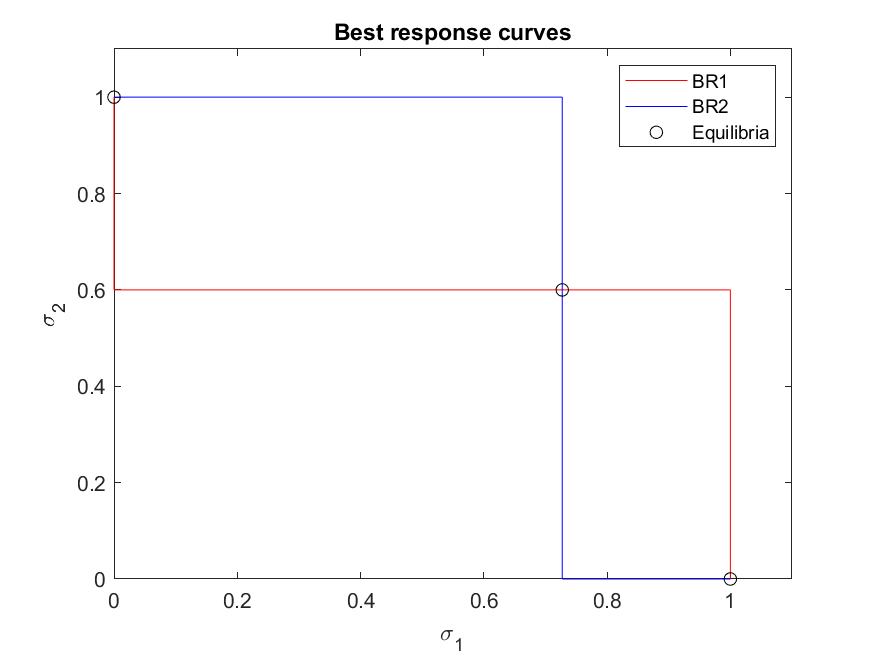
\includegraphics{fig1}
% make graph

\section{Question 4}
None of the pure strategies are dominated by any other pure strategies. So, all strategies are 1-rationalizable.

If player 1 chooses A, player 2's best response is b, and player 1's best response is B, and player 2's best response is c, and player 1's best response is C, and player 2's best response is d, and player 1's best response is D, and player 2's best respoonse is a, and player 1's best response is A. This loop continues endlessly. Also, if player 1 chooses E, then player 2 will choose e, and player 1 will choose E, and the loop will continue. Thus, A,B,C,D,E,a,b,c,d,e are all rationalizable. 

\section{Question 5}
\subsection{Part A}
$N = \{ 1,2\}, S_i = \{\text{seek},\text{not} \}$, $u(s_i,s_{-i}) = \begin{cases} R-c, s_i = \text{seek}, s_{-i} = \text{not} \\ r-c, s_i = s_{-i} = \text{seek} \\0, s_i = \text{not} \end{cases}.$
\subsection{Part B}
If $c>R$, then even in the best case scenario, if the firm does seek approval they will receive less return $R-c<0$ than if they did not seek approval. So, they will never seek approval. Similarly, if $c<r,$ then even in the worst case scenario the firm will receive more return for seeking approval than not seeking approval $(c-r>0)$. Thus, they will always seek approval. If $c=r,$ then the firm has a chance at receiving a return $R-c$ by seeking approval with no downside $(r-c=0)$ to not seeking approval, so the firm will seek approval. Similarly, if $c=R,$ the firm has no upside to trying to seek approval but has downside in doing so $R-c=0,r-c<0$ so the firm will not seek approval. The more 'interesting' region of parameterization for $c$ is $(r,R)$.

Let $c \in (r,R)$. If the first firm believes that the second firm is not seeking approval, their best response is to seek approval. The second firm's best response is to then not seek approval, and the cycle repeats ad infinitum. If, instead, the first firm believes that the second is seeking approval, the first firm will not seek approval, so the second will seek approval, and the cycle continues endlessly. Thus, both seek and not are rationalizable strategies for both firms.

A firm will be indifferent between seeking or not if they expect the other firm's probability of seeking to satisfy the following: $p(r-c) + (1-p)(R-c) = p_1(0) + (1-p_1)(0) = 0 \Rightarrow p = \frac{R-c}{R-r}.$ For any belief that the other firm's probability of seeking approval is less than this value, the optimal response is to seek approval, and for any belief that the other firm's probability of seeking approval is greater than this value, the optimal response is to not seek approval. 

To summarize, for $c\leq r,$ the strictly dominant strategy is to seek approval for the drug, while for $c\geq R$ seeking approval is strictly dominated. For $c \in (r,R)$ the optimal strategy depends upon the beliefs of the other firms, with indifference between seeking and not seeking approval at the belief that the other firm will seek approval with probability $\frac{R-c}{R-r}$ and probabilities lower and higher result in the dominant strategy being to seek and not seek approval, respectively. The best response graph for this is drawn below.

% make graph
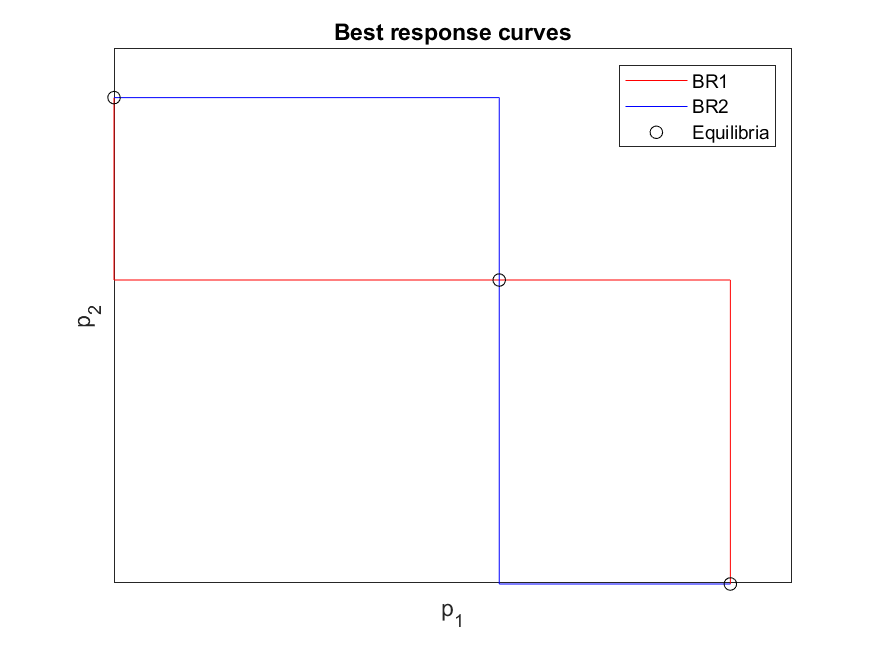
\includegraphics{fig2}
\end{document}
